\documentclass[12pt,a4paper, twosite]{article}
\usepackage[utf8]{inputenc}
\usepackage[T1]{fontenc}
\usepackage{graphicx}
\usepackage{grffile}
\usepackage{longtable}
\usepackage{wrapfig}
\usepackage{rotating}
\usepackage[normalem]{ulem}
\usepackage{amsmath}
\usepackage{textcomp}
\usepackage{amssymb}
\usepackage{capt-of}
\usepackage{hyperref}
\usepackage[left=2.00cm, right=2.50cm, top=2.50cm, bottom=2.00cm]{geometry}
\usepackage{fancyhdr}
\usepackage[spanish]{babel}
\fancyhead[RO,LE]{\thepage}
\fancyhead[LO]{\emph{\uppercase{\leftmark}}}
\fancyfoot{}
\renewcommand{\headrulewidth}{1.0pt}
\pagestyle{fancy}
\date{\today}
\title{IEEE-830}
\hypersetup{
	pdfborder={0 0 0},
	pdfauthor={fasdas ads d},
	pdftitle={IEEE-830},
	pdfkeywords={hola},
	pdfsubject={hola mundo},
%	pdfcreator={Emacs 26.2 (Org mode 9.1.9)}, 
	pdflang={Spanish}}


\begin{document}
	\begin{titlepage}
		\maketitle
		
	\end{titlepage}

\section*{Historial de cambios  }
crear tabla de el versionado de los cambios 

\newpage
	\tableofcontents	
\newpage
	\section{Introducción}
	\label{sec:org60390fa}



	
	\subsection{Propósito}
	\label{sec:org434c3ef}
	Este documento presenta una especificación de requerimientos de software para unsistema de  posicionamiento de antena. Este dispositivo generalmente se conoce como rotador. Este tiene dos ejes, uno denominado azimuth,y el otro altura o elevación. 
	 
	Esta dirigido a técnicos, profesionales y operarios que intervengan en los sistemas de apuntamiento que posee el IAR.   

	
	
	\subsection{Ámbito del sistema}
	\label{sec:org12e44a1}
	Este sistema, se desarrolla como un subsistema del interferómetro MIA(https://www.iar.unlp.edu.ar/slider/observatorio/), y el proyecto de construcción de estaciones terrenas. Se utilizar para realizar el apuntamiento de radiofuentes, y el seguimiento de satelites en forma automática.  El nombre del sistema rotador sera ROT\_IAR. Adicionalmente, tiene espectativas de escalar, y realizar una producción en serie. 
	
	
	\subsection{Definiciones, Acrónimos y Abreviaturas}
	\label{sec:orgb158e36}
	
	ver los acrónimos al terminar el documento 
	
	
	\subsection{Referencias}
	\label{sec:org62711e0}
	ver tesis, y plan de trabajo ! 
	
	\subsection{Visión general del documento}
	\label{sec:orgdaca22c}
	
	Este documento se realiza siguiendo el estándar IEEE Std. 830-1998
	
	
	\section{Descripción general del documento}
	\label{sec:orgc1c4017}
	
	\subsection{Perspectiva del producto}
	\label{sec:org24980a8}
%	El proyecto aquí especificado es independiente de otros sistemas y no tiene relación con otros productos
	El software es parte de un sistema mayor, denominado interferómetro MIA y estaciones terrenas. Este sistema de apuntamiento, se adicionara al sistema mecánico de la antena que esta en fase de construcción. Este sistema, realizará el apuntamiento de antena, y este según el proyecto(MIA o estaciones terrenas) es automático o manual. El diagrama en bloques del sistema se muestra en la figura \ref{fig:diagramaBloques}. 
	
	 El presente documento describe los requerimientos de software del bloque single board computer, y las interfaces del sistema que se observa en la figura  \ref{fig:diagramaBloques}. 
	\begin{figure}[h!]
		\centering
		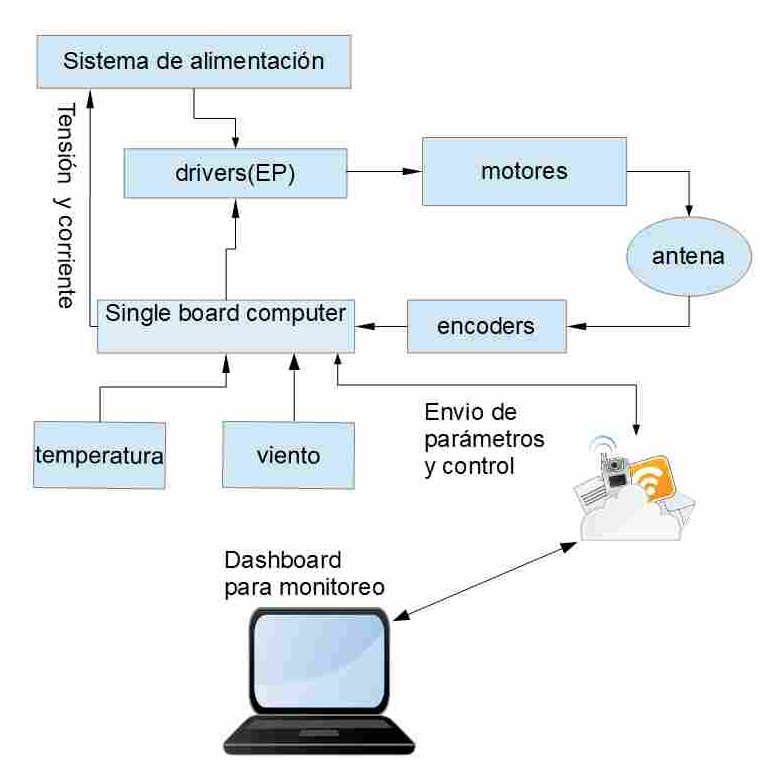
\includegraphics[scale=0.5]{bloquesInt.jpg}
		\caption{Diagrama en bloques del sistema}
		\label{fig:diagramaBloques}
	\end{figure}
	\subsection{Funciones del producto}
	\label{sec:orgaf51da6}
	\begin{enumerate}
		\item control de posición
		\item Servidor web embebido 
		\item Compatible con el software Gpredict y Stellarium, y scripts de antenas principales 
		\item Reinicio del en forma remota  
		\item Interrupción de operación en caso de condiciones climáticas adversas. 
		\item información de la operación y estado actual del sistema(tracking, untracked, y cenit). 
	\end{enumerate}
	
	\subsection{Características de los usuarios}
	\label{sec:orga40b0ee}
	Los usuarios serán técnicos, operarios y profesionales con conocimiento y experiencia en los sistemas de apuntamiento y manejo de rotadores. 
	\subsection{Restricciones}
	\label{sec:org5ca5790}
	
	
	\begin{itemize}
		
		\item Lenguaje python3 por cuestiones de compatibilidad de scripts de manejo principal de las antenas.
		\item El software debe estar bajo control de versiones.  
%		\item  se debe realizar un informe de avance por cada requerimiento que se cumple 
	\end{itemize}
	
	
	\subsection{Suposiciones y dependencias}
	\label{sec:org0ae23fe}
	Se supone que se cuenta con los scripts del manejo de las antenas principales 
	
	Se cuenta con los encoders y motores seleccionados. 
	
	
	\subsection{Requisitos futuros}
	\label{sec:org33cfcdb}
	El sistema posea control de velocidad 
	
	El diseño electrónico escalable, y realizable en una cadena de producción.  
	
	El sistema debe poseer autocalibración en base al sol o la luna(esto dependerá del horario en que se realice la autocalibración).  
	
	El sistema tendra que identificarse mediante algún código alfanumérico
	
	
	\section{Requisitos específicos}
	\label{sec:org40573d1}
	
	
	\subsection{Interfaces externas}
	\label{sec:orgfd5391f}
	\begin{itemize}
		\item El sistema se comunicara con una red local mediante cable ethernet con conector RJ45
		\item El sistema se conecta con un sensor de temperatura DHT11 mediante onewire. 
		\item El sistema se conecta con los drivers de los motores mediante puertos que posean salida PWM. 
		\item Los encoders serán conectados en un puerto analógico digital. 
		\item El sistema de medición del viento se realizará con un anemómetro, y se conectará a un puerto analógico digital
		\item Se realizará un PCB que se acople al single board computer mecánicamente con borneras, donde se indique mediante serigrafia donde se conecta. Esta serigrafia será: 
		\begin{itemize}
			\item EP1: motor de azimuth 
			\item EP2: motor de altura
			\item ENC1: encoder de azimuth 
			\item ENC2: encoder de altura 
			\item VTO: anemómetro 
			
		\end{itemize} 
		
	\end{itemize}
	
	\subsection{Funciones}
	\label{sec:org307bb59}
	\subsection{Control de posición}
	\begin{enumerate}
		\item El sistema debe realizar un control a lazo cerrado mediante la lectura de los encoders cada 100 ms, mientras se encuentre encendido.
		\item Debe poder manejar el sistema de coordenadas ecuatorial y altacimutal, y realizar las transformaciones matemáticas correspondientes 
		\item El control se realiza mediante un control on/off. 
		\item El sistema tiene tres estados: 
			\begin{enumerate}
				\item TRACKING: seguimiento de satelite o radiofuente. Debe ser independiente del tipo de objeto estelar a seguir
				\item UNTRACKING: no se esta realizando ningún tipo de seguimiento 
				\item CENIT: posición de reposo de la antena
			\end{enumerate}
	
	\end{enumerate}
	\subsection{Servidor Web embebido}
	\begin{enumerate}
		\item El servidor informa del estado estado actual(TRACKING, UNTRACKING, CENIT). Además informa el estado de corriente en ampere, tensión de operación en volts, viento en km/h y temperatura en grados centigrados 
		\item Debe realizar movimientos de la antena a demanda del operador 
		\item Debe poseer una función de calibración para los encoders e informar su lectura 
		\item Debe poseer mecanismo de POST/GET para consulta de estados mediante consola. 
		\item Se deben utlizar los scripts de las antenas principales. Esto implica la realización en python del servidor web embebido
		\item Debe poseer mecanismo para realizar el gráfico de tensión,corriente, viento y temperatura, durante los últimos 10 minutos y verse en pantalla.
	\end{enumerate}

\subsection{Conexión con software externo}
	\begin{itemize}
		\item Debe usarse Stellarium y Gpredict para realizar seguimientos de radiofuentes o satelites
		\item Se deben utilizar sockets y configuraciones especificas para cada software. 
	\end{itemize}


\subsection{Entorno de operación y mantenimiento}
\begin{enumerate}
	\item El sistema debe realizar la medición de temperatura y viento cada 2 minutos 
	\item Si la velocidad supera los 50 km/h durante diez, debe llevar la antena a su posición de cenit, independientemente de su estado actual. Si estaba en cenit, debe quedarse alli hasta que la velocidad del viento sea inferior a 50 km/h durante al menos 10 minutos
	\item Debe almacenar los datos desde las 5AM de un dia, hasta las 5AM del dia siguiente, y enviar la información a un servidor dentro de la institución. Estos datos tienen el siguiente formato: 
	\begin{itemize}
		\item timestamp , tensión[V], corriente[A], temperatura[°C] , viento[KM/H], ESTADO, posición\_azimuth,posición\_altura 
	\end{itemize}  
	La hora de envio será las 5 AM de cada dia. El nombre del archivo enviado es en formato txt, y posee el siguiente formato de nombre: 
	\begin{itemize}
		\item IAR\_MIA\_FECHA\_ANTENA.txt 
	\end{itemize} 
	\item El archivo debe ser procesado y almacenado en un directorio dentro del repositorio de la institución mediante un script y realizar un analisis de los parámetros que reciben. En caso de anomalia, debe alertar a los operadores mediante el envio de un SMS o mail.  
\end{enumerate}

	\subsection{Requisitos de rendimiento}
	\label{sec:org94bc543}
	
	El sistema, debe soportar hasta 20 conexiones simultaneamente. Si esta en estado TRACKING, al conectarse simultaneamente otro operador, debe informarsele que debe esperar que finalice la operación. 
	
	\subsection{Restricciones de diseño}
	\label{sec:org49fe900}
	
	Se debe realizar el servidor web embebido en python, para tener compatibilidad con los scripts de manejo de las antenas principales de la institución. 
	
	\subsection{Atributos del sistema}
	\label{sec:orgd0babc0}
	Debe tener la capacidad de actualizar el software manualmente mediante red local, si se desea agregar otro software aparte de Gpredict y Stellarium (por ejemplo orbitron)
	
\end{document}